\scanpage{47}\mspage{46}
\margin{\figure{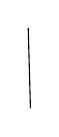
\begin{tikzpicture}[x=1pt,y=1pt]\draw (0,0) -- (.8,-29);\end{tikzpicture}}}
\uline{Corollaire} \inserted{(Cas ultratopologique)} Supposons que la top. de $J'$ soit quotient de celle de $J$, \deleted{Alors} i.e. $\varphi^{\unsure{*|\star}}:J'\longrightarrow \deleted{\unsure{I}}J$ submersif. Alors $\varphi$ aussi.

\uline{Corollaire} \inserted{(\unsure{Ultratopologies})} Supposons $\varphi^*$ submersif \unsure{à|;} fibres $0$-connexes -- alors $\varphi$ \unsure{item|idem|itou}. Supposons $\varphi^*$ \deleted{\unsure{aussi}} homotopiquement propre i.e. les $\varphi^{{*\unsure{)|\prime}}^{-1}}(J_{\deleted{\unsure{<|\leq}}\unsure{\leq|<}x})$ ``faiblement contractiles''. \deleted{\unsure{(quasi-hom}} Alors kif-kif pour $\varphi\deleted{^{\unsure{*|\leq}}}$.

On est ramené à prouver que si $I$ admet un plus grand élément \inserted{$x$} (donc est f.c.)\inserted{$x\notin J$}, alors $I'$ est f. \unsure{kontractile|contractile}. Mais considérons l'unique élément \inserted{$x'$} de $I'$ au dessus de $x$, prouvons que c'est un plus grand élément. En effet, comme $x'\in I'\setminus{\unsure{U|u|n}}'$, son adhérence \unsure{pour} $\overline{{\unsure{\mathcal{T}|\tau}}'}$, et pour $\unsure{\overline{\mathcal{T}}|\widetilde{\mathcal{T}}}$, est la \unsure{$=$}, donc c'est tout. OK !

\uline{Corollaire} \inserted{(Ultratopologies)} Si $\varphi^*$ est homotopiquement propre à fibres \deleted{\unsure{fib}} faiblement contractibles (donc une équivalence d'homotopie faible universelle), \unsure{item|idem} pour $\varphi$.

